   \documentclass[%
oneside,                 % oneside: electronic viewing, twoside: printing
final,                   % draft: marks overfull hboxes, figures with paths
10pt]{article}

\listfiles               %  print all files needed to compile this document

\usepackage[a4paper, total={6in, 8in}]{geometry}
\usepackage[totoc]{idxlayout}   % for index in the toc
\usepackage[nottoc]{tocbibind}  % for references/bibliography in the toc

\usepackage{relsize,makeidx,color,setspace,amsmath,amsfonts,amssymb}
\usepackage[table]{xcolor}
\usepackage{bm,ltablex,microtype}
\usepackage{comment} 
\usepackage[pdftex]{graphicx}

\usepackage{fancyvrb} % packages needed for verbatim environments

\usepackage[T1]{fontenc}
%\usepackage[latin1]{inputenc}
\usepackage{ucs}
\usepackage[utf8x]{inputenc}

%extra space in tabs
\usepackage{array}
\setlength{\extrarowheight}{.5ex}


\usepackage{lmodern}         % Latin Modern fonts derived from Computer Modern


\usepackage{pgfplotstable, booktabs}

\pgfplotstableset{
    every head row/.style={before row=\toprule,after row=\midrule},
    every last row/.style={after row=\bottomrule}
}


%Test subsubsubscetion
\usepackage{titlesec}
\usepackage{hyperref}

\titleclass{\subsubsubsection}{straight}[\subsection]

\newcounter{subsubsubsection}[subsubsection]
\renewcommand\thesubsubsubsection{\thesubsubsection.\arabic{subsubsubsection}}
\renewcommand\theparagraph{\thesubsubsubsection.\arabic{paragraph}} % optional; useful if paragraphs are to be numbered

\titleformat{\subsubsubsection}
  {\normalfont\normalsize\bfseries}{\thesubsubsubsection}{1em}{}
\titlespacing*{\subsubsubsection}
{0pt}{3.25ex plus 1ex minus .2ex}{1.5ex plus .2ex}

\makeatletter
\renewcommand\paragraph{\@startsection{paragraph}{5}{\z@}%
  {3.25ex \@plus1ex \@minus.2ex}%
  {-1em}%
  {\normalfont\normalsize\bfseries}}
\renewcommand\subparagraph{\@startsection{subparagraph}{6}{\parindent}%
  {3.25ex \@plus1ex \@minus .2ex}%
  {-1em}%
  {\normalfont\normalsize\bfseries}}
\def\toclevel@subsubsubsection{4}
\def\toclevel@paragraph{5}
\def\toclevel@paragraph{6}
\def\l@subsubsubsection{\@dottedtocline{4}{7em}{4em}}
\def\l@paragraph{\@dottedtocline{5}{10em}{5em}}
\def\l@subparagraph{\@dottedtocline{6}{14em}{6em}}
\makeatother

\setcounter{secnumdepth}{4}
\setcounter{tocdepth}{4}
%end of subsubsusbbu


% Hyperlinks in PDF:
\definecolor{linkcolor}{rgb}{0,0,0.4}
\usepackage{hyperref}
\hypersetup{
    breaklinks=true,
    colorlinks=true,
    linkcolor=linkcolor,
    urlcolor=linkcolor,
    citecolor=black,
    filecolor=black,
    %filecolor=blue,
    pdfmenubar=true,
    pdftoolbar=true,
    bookmarksdepth=3   % Uncomment (and tweak) for PDF bookmarks with more levels than the TOC
    }
%\hyperbaseurl{}   % hyperlinks are relative to this root

\setcounter{tocdepth}{2}  % levels in table of contents

% --- fancyhdr package for fancy headers ---
\usepackage{fancyhdr}
\fancyhf{} % sets both header and footer to nothing
\renewcommand{\headrulewidth}{0pt}
\fancyfoot[LE,RO]{\thepage}
% Ensure copyright on titlepage (article style) and chapter pages (book style)
\fancypagestyle{plain}{
  \fancyhf{}
  \fancyfoot[C]{{\footnotesize \copyright\ 1999-2018, "Computational Physics I FYS3150/FYS4150":"http://www.uio.no/studier/emner/matnat/fys/FYS3150/index-eng.html". Released under CC Attribution-NonCommercial 4.0 license}}
%  \renewcommand{\footrulewidth}{0mm}
  \renewcommand{\headrulewidth}{0mm}
}
% Ensure copyright on titlepages with \thispagestyle{empty}
\fancypagestyle{empty}{
  \fancyhf{}
  \fancyfoot[C]{{ }}
  \renewcommand{\footrulewidth}{0mm}
  \renewcommand{\headrulewidth}{0mm}
}

\pagestyle{fancy}


% prevent orhpans and widows
\clubpenalty = 10000
\widowpenalty = 10000

% --- end of standard preamble for documents ---


% insert custom LaTeX commands...

\raggedbottom
\makeindex
\usepackage[totoc]{idxlayout}   % for index in the toc
\usepackage[nottoc]{tocbibind}  % for references/bibliography in the toc
\usepackage{listings}
\usepackage[normalem]{ulem} 	%for tables
\useunder{\uline}{\ul}{}
\usepackage{hyperref}
\usepackage[section]{placeins} %force figs in section

\usepackage{natbib}

\usepackage[toc,page]{appendix} % appenix
\usepackage{amsmath} % split in align
\usepackage{multirow} %multirow


%-------------------- end preamble ----------------------

\begin{document}

% matching end for #ifdef PREAMBLE

\newcommand{\exercisesection}[1]{\subsection*{#1}}


% ------------------- main content ----------------------



% ----------------- title -------------------------

\thispagestyle{empty}

\begin{center}
{\LARGE\bf
\begin{spacing}{1.25}
VMC: Effects of Importance Sampling and Jastrow factor on error estimates %
\end{spacing}
}
\end{center}

% ----------------- author(s) -------------------------

\begin{center}
{\bf Johan Nereng}
\end{center}

    \begin{center}
% List of all institutions:
\centerline{{\small Department of Physics, University of Oslo, Norway}}
\end{center}
    
% ----------------- end author(s) -------------------------

% --- begin date ---
\begin{center}
Spring, 2020
\end{center}
% --- end date ---

\vspace{3cm}
\vspace{3cm}
\begin{abstract}
This project aimed to examine using Vartiational Monte Carlo (VMC) in making an estimate, $\bar E$, of the ground state energy, $E_0$, of a trapped, hard sphere Bose gas. The error of the energy estimate was evaluated by using the sample error with "blocking", $\hat \sigma$. This method accounts for sample correlation, which was concluded to be necessary as the raw sample error was largely deceptive. Two approaches to the sampling scheme involved in the Metropolis algorithm were used, "Importance Sampling" and the "Brute Force" approach. "Importance sampling" was found to equilbrate the system faster than the "Brute Force" approach, albeit only for suitable values of $\Delta t$. Several other parameters, such as the number of particles, $N$ and the value $\alpha$ was observed to affect the suitability of different $\Delta t$ values. Increases in particle number, $N$, was generally observed to increase $\hat \sigma$; after $2^{18}$ Monte Carlo cycles, $\hat \sigma \sim 10^3$ ($N=10$) increased to $\sim 10^2$ ($N=50$) and $\sim 10^{-1}$ ($N=100$), both with and without the Jastrow factor, which accounts for particle-particle correlation.  Incorporating the Jastrow factor was concluded to have an increasing effect on the average estimated energy per particle $\bar E /N$ as $N$ increased, from $\bar E/N\approx2.45\approx$ constant for all values of $N$, to $4.55$ ($N=50$) and $2.66$ ($N=100$). This impact dependence was further verified by qualitative comparison of one-body densities. 
\end{abstract}


\newpage


\textit{\textbf{Author's comments:} I struggled a lot to finish this project, both because of the COVID situation and because I was ill for several weeks. However, I found that the biggest challenge was to find a suitable level of detail and robustness in the results I presented. I've spent days looking at charts and numbers, and managed to convince myself of all sorts of connections that was not really of any importance, all because I never limited the scope of my examination. I am very grateful to Doctoral Research Fellow Øyvind Sigmundson Schøyen for answering my many questions and for repeatedly trying to remind me that everything did not have to be perfect. In the end, I had to remove a lot of results, as well as produce new ones in order to support the direction my project took. The biggest lesson I've learned from this is that I need to have concrete goals for my work before getting in to deep. In the future I will aim to concertize and narrow the scope of my work after having familiarized myself with the theoretical ground work, instead of doing so while describing results.}
\newpage


\section{Introduction}
Variational Monte Carlo (VMC) is widely used to approximate ground states in quantum systems, and may be applied where other methods, such as the mean field Gross-Pitaevskii equation, fails. For VMC methods, the accuracy of the estimated ground energy is largely dependent on factors such as the number of Monte Carlo cycles used, and the number of parameters involved in tuning the simulation. However, one of the most significant error reducing factors is the application of the Jastrow factor, which accounts for particle-particle correlation. In this project the impact of including the Jastrow factor in a hard sphere Bose gas is studied for various numbers of particles, using an improved error estimation method called "blocking". Without "blocking", which addresses the correlation between samples in the computer generated data, the error estimate tends to be overly optimistic, and may - when not careful - lead to results which implies entirely wrong conclusions. Two VMC methods are compared in this project, the "brute force" implementation of the Metropolis algorithm, and in improvement on it's sampling scheme called "Importance Sampling". Where the "brute force" suggests particle moves in entirely random directions, "Importance Sampling" uses the drift force acting on a particle to suggest more likely moves, thus suggesting moves that are more likely to be accepted by the Metropolis algorithm. 

First, the system of Bose gas is introduced, including the expressions for the local energy, $E_L$ and drift force $F$. Then, analytic expressions for $E_L$ and $F$ are derived, both with and without the Jastrow factor. The variational principle, which is the theoretical basis for approximating $E_0$ by an integral over $E_L$, is then introduced. Application of this principle relies on approximating the integral by a sum over $E_L$ for a number of system states and their corresponding probability. In order to generate these local energies and probabilities, the Metropolis algorithm is used. The algorithm is based on initiating a random state of $N$ particles, before moving one particle at a time, and either rejecting or accepting each proposed new state according to a sampling rule. Having outlined this algorithm, the improved sampling method called "Importance Sampling" is briefly explained. In order to optimize $\alpha$ when including the Jastrow factor, the Gradient Descent method for minimizing a cost function is outlined, using the local energy as a cost function dependent on $\alpha$. Finally, the error analysis is presented, including the "blocking" method and the "automated blocking" algorithm from \citep{Jonsson}.

 
In order to write this project paper and the code required to produce the results, I used a variety of tools, including: C++, Python 3.7.7, NumPy \cite{numpy}, as well as a number of books, web-pages and articles - of which most are listed under 
 \hyperref[refer]{references}. All the code required to reproduce the results may be found on my \href{https://github.com/johanere/FYS4411}{github page }.  
 
\section{Material and methods} \label{theory}
\subsection{System: Boson gas}
The system consists of $N$ Bosons in an harmonic spherical (S) ($\omega_{ho}^2=\omega_z^2$) or elliptical (E) ($\omega_{ho}^2 \neq \omega_z^2$) trap \eqref{trap_eqn};
\begin{equation}
 V_{ext}(\mathbf{r}) = 
 \Bigg\{
 \begin{array}{ll}
	 \frac{1}{2}m\omega_{ho}^2r^2 & (S)\\
 \strut
	 \frac{1}{2}m[\omega_{ho}^2(x^2+y^2) + \omega_z^2z^2] & (E)
 \label{trap_eqn}
 \end{array}
 \end{equation}, 
 where $\omega_{ho}$ and  $\omega_z$ are trap frequencies in the $xy$ plane and $z$ direction respectively. The characteristic length of the trap is defined $a_{ho}=(\hbar /m \omega_{ho})^{1/2}$, while the ratio of the trap lengths in the $xy$ plane and the $z$ direction is $a_{ho}/a_z=(\omega_z/\omega_{ho})^2=\sqrt{\lambda}$, which will be used when scaling the system. The Hamiltonian of the system is given by
\begin{equation}
     H = \sum_i^N \left(\frac{-\hbar^2}{2m}{\bigtriangledown }_{i}^2 +V_{ext}({\mathbf{r}}_i)\right)  +
	 \sum_{i<j}^{N} V_{int}({\mathbf{r}}_i,{\mathbf{r}}_j),
	 \label{eq:hamiltonian}
 \end{equation}
where the Boson interaction is given by the repulsive force prohibiting particles to come within a distance $a$ of other particles;
\begin{equation}
 V_{int}(|\mathbf{r}_i-\mathbf{r}_j|) =  \Bigg\{
 \begin{array}{ll}
	 \infty & {|\mathbf{r}_i-\mathbf{r}_j|} \leq {a}\\
	 0 & {|\mathbf{r}_i-\mathbf{r}_j|} > {a}
 \end{array}
 \end{equation}

In order to evaluate the ground-state energy, a trial wave function (TWF) is used \eqref{eq:trialwf}, where $\alpha$ and $\beta$ are variational parameters used to tune the wave function towards ground-state (more under a the \hyperref[S:VMC]{section on VMC}).

\begin{equation}
 \Psi_T(\mathbf{r})=\Psi_T(\mathbf{r}_1, \mathbf{r}_2, \dots \mathbf{r}_N,\alpha,\beta)
 =\left[
    \prod_i g(\alpha,\beta,\mathbf{r}_i)
 \right]
 \left[
    \prod_{j<k}f(a,|\mathbf{r}_j-\mathbf{r}_k|)
 \right],
 \label{eq:trialwf}
\end{equation}
Where
\begin{equation}
    g(\alpha,\beta,\mathbf{r}_i)= \exp{[-\alpha(x_i^2+y_i^2+\beta z_i^2)]}.
 \end{equation}
is the non-interactive part of the wave function, and 
\begin{equation}
    f(a,|\mathbf{r}_i-\mathbf{r}_j|)=\Bigg\{
 \begin{array}{ll}
	 0 & {|\mathbf{r}_i-\mathbf{r}_j|} \leq {a}\\
	 (1-\frac{a}{|\mathbf{r}_i-\mathbf{r}_j|}) & {|\mathbf{r}_i-\mathbf{r}_j|} > {a}.
 \end{array}
 \end{equation}
the interactive part, or the Jastrow correlation factor.  



\subsubsection{Local energy and drift force}
When using the Monte Carlo methods described later, the particles will be moved one at a time. After each such move, the local energy \eqref{eq:locale} will be evaluated, and used to calculate the ground energy of the system. 
 
\begin{equation}
    E_L(\mathbf{r})=\frac{1}{\Psi_T(\mathbf{r})}H\Psi_T(\mathbf{r}).
    \label{eq:locale}
 \end{equation}
 
As the algorithms will involve repeatedly calculating the local energy, every reduction of floating point operations (FLOPs) involved in doing so will lead to a significant speed up - which is why an analytical expression for the local energy is desirable. As will be discussed more under \hyperref[importance_sampling]{importance sampling}, the drift force of the  particles are also needed;

\begin{equation}
F_i = \frac{2\nabla \Psi_T}{\Psi_T}
\end{equation} 

\subsubsubsection{Local energy and drift force: Non-interacting boson sphere}
For a spherical harmonic oscillator with no interaction between particles, $a=0$ and $\beta = 1$, the TWF \eqref{eq:trialwf} reduces to;
\begin{equation}
\Psi_T (\bm r)= \left[
    \prod_i g(\alpha,\beta,\mathbf{r}_i)
 \right]
\end{equation}

Thus simplifying the expression needed for the local energy \eqref{eq:locale} to;
\begin{equation*}
    E_L(\mathbf{r}) =\frac{1}{ 
    \prod_i g(\alpha,\beta,\mathbf{r}_i)
}  \sum_i^N \left(\frac{-\hbar^2}{2m}{\nabla }_{i}^2 +\frac{1}{2}m\omega_{ho}^2r^2 \right)  \left[
    \prod_i g(\alpha,\beta,\mathbf{r}_i)
 \right]
 \end{equation*}

which leads to (see \hyperref[APP_2:le_1]{Appendix 1: Analytic local energy, non-interacting spherical}) the following expression when using natural units, $\hbar = c = 1 $, and unity mass, $m=1$;

\begin{equation}
        E_L(\mathbf{r}) =  \alpha d N + \left( - 2 \alpha^2    + \frac{1}{2} \omega_{ho}^2\right)  \sum_i^N r_i^2 .
\label{eq:locale_analytic_1}
\end{equation}

With drift force;
\begin{equation}
F_i = \frac{2\nabla \Psi_T}{\Psi_T}= -4\alpha \mathbf{r}_i 
\end{equation}
 
\subsubsubsection{Local energy and drift force: interacting boson sphere with elliptic trap}
Next, an analytic expression for the local energy of an elliptical trap with particle interaction, $\beta\neq 1$ and $a \neq 0$, is required. In order to derive it, the TWF \eqref{eq:trialwf} is re-written. First, the non-interactive part; 
\begin{equation*}
    g(\alpha,\beta,\mathbf{r}_i) = \exp{\left[-\alpha(x_i^2+y_i^2+\beta
    z_i^2)\right]}= \phi(\mathbf{r}_i) = \phi_i.
\end{equation*}

Secondly, the interactive part;

\begin{equation}
\prod_{i<j} f(r_{ij})= \exp{\left(\sum_{i<j}u_{jk}\right)}
\end{equation}
Where $u_{jk}=\ln{f(r_{ij})}$, using the shorthand notation $r_{ij}=|\mathbf{r}_i-\mathbf{r}_j|$. Thus, the WTF \eqref{eq:trialwf} is expressed as;

\begin{equation*}
\Psi_T(\mathbf{r})=\left[
    \prod_i \phi_i
\right]
\exp{\left(\sum_{j<k}u_{jk}\right)}
\end{equation*}
Which means that the local energy, using natural units and unity mass as before, \eqref{eq:locale} can be written as

\begin{equation}
    E_L(\mathbf{r}) =\frac{1}{ 
    \left[
    \prod_i \phi_i
\right]
\exp{\left(\sum_{j<k}u_{jk}\right)}
}  \sum_i^N \left(\frac{1}{2}{\nabla }_{i}^2 +V_{ext}(\bm r_i) \right)  \left[
    \prod_i \phi_i
\right]
\exp{\left(\sum_{j<k}u_{jk}\right)}
\end{equation}
where (see \hyperref[APP_2:le_2]{Appendix 1: Analytic local energy, interacting elliptical})
\begin{align}
\begin{split}
\frac{1}{\Psi_T(\mathbf{r})} \nabla_k^2\Psi_T(\mathbf{r}) 
&=
\frac{\nabla_k^2 \phi_k}{\phi_k} + 2  \frac{\nabla_k \phi_k}{\phi_k} \sum_{l\ne k}\frac{\bm r_k - \bm r_l}{r_{kl}}  u'_{kl}  \\
&+  \sum_{j\ne k} \sum_{l\ne k} \frac{(\bm r_k - \bm r_l)(\bm r_k - \bm r_j)}{r_{kj} r_{kl} }  u'_{kj}  u'_{kl} \\
&+ \sum_{l\ne k} \left(   u{''}_{kl} + \frac{2}{r_{kl}}   u'_{kl} \right)
\end{split}
\end{align}
Thus
\begin{align}
\begin{split}
    E_L(\mathbf{r}) &= \frac{1}{2}\sum_{k=1}^N \left(\frac{\nabla_k^2 \phi_k}{\phi_k} 
    + 2 \frac{\nabla_k \phi_k}{\phi_k} \sum_{l\ne k}\frac{\bm r_k - \bm r_l}{r_{kl}}  u'_{kl}
    +  \right( \sum_{j\ne k}  \frac{(\bm r_k - \bm r_j)}{r_{kj} }  u'_{kj} \left)^2
    +  \sum_{l\ne k} \left(   u{''}_{kl} + \frac{2}{r_{kl}}   u'_{kl} \right) +V_{ext}(\bm r_i) \right)  
\end{split}
\end{align}
Where
\begin{align*}
\frac{\nabla_k \phi_k}{\phi_k} &=-2\alpha (x_k \vec e_1 + y_k \vec e_2 + \beta z_k \vec e_3), \\
\frac{\nabla_k^2 \phi_k}{\phi_k}&=-2\alpha (d-1+\beta)+4\alpha^2 (x_k   + y_k^2 + \beta^2 z_k^2), \\
\frac{\partial u_{kl}}{\partial r_{kl}}&= \frac{a}{r_{kl}(r_{kl}-a)}, \\
\frac{\partial^2 u_{kl}}{\partial r^2_{kl}}&= \frac{a^2-2ar_{kl}}{r_{kl}^2(r_{kl}-a)^2}
\end{align*}
And drift force;
\begin{equation*}
F_k = \frac{2\nabla \Psi_T}{\Psi_T}= 2 \left(\ \frac{\nabla_k \phi_k}{\phi_k} + \sum_{l\ne k}\nabla_k u_{kl} \right) 
\end{equation*}
Where $\nabla_k u_{kl}=\frac{\bm r_k - \bm r_l}{r_{kl}}\frac{\partial u_{kl}}{\partial r_{kl}}$

\subsubsection{Scaling the system}
As in \citep{VMCHJ} and \citep{VMCdubois}, the system is scaled using $a/a_{ho}=0.0045$, with units of length of $a_{ho}$, $r\rightarrow r/a_{ho}$ and energy units of $\hbar \omega_{ho}$. This means that $\nabla_i\rightarrow \frac{1}{a_{ho}} \nabla_i$, thus the Hamiltonian \eqref{eq:hamiltonian} can be written as;

\begin{align}
\begin{split}
  H &= \sum_i^N \left(\frac{-\hbar^2}{2m}\frac{1}{a_{ho}^2} \nabla_i^2 +
  \frac{1}{2}m \omega_{ho}^2a_{ho}^2(x^2+y^2+ \frac{\omega_z^2}{\omega_{ho}^2}z^2]  
  \right)  +
	 \sum_{i<j}^{N} V_{int}({\mathbf{r}}_i,{\mathbf{r}}_j) \\
	 &= \sum_i^N \left(\frac{-\hbar^2}{2m}\frac{m \omega_{ho}}{\hbar} \nabla_i^2 +
  \frac{1}{2}m   \omega_{ho}^2 \frac{\hbar}{m \omega_{ho}}(x^2+y^2+ \frac{\omega_z^2}{\omega_{ho}^2}z^2)  
  \right)  +
	 \sum_{i<j}^{N} V_{int}({\mathbf{r}}_i,{\mathbf{r}}_j) \\
	  &= \sum_i^N \frac{1}{2} \left(- \nabla_i^2 +x^2+y^2+ \lambda^2 z^2  
  \right)  +
	 \sum_{i<j}^{N} V_{int}({\mathbf{r}}_i,{\mathbf{r}}_j) \label{eq:scaled_H}
\end{split}
\end{align}
\subsection{Variational Monte Carlo} \label{S:VMC}
There are various methods available to circumnavigate having to directly solve the Schrõdinger equation in order to find the eigenpair of the system we are looking for. An important underlying principle for the methods employed in this project is the variational principle \citep{Griffiths95}[p.256.]; 

\begin{equation}
E_0\leq E[H]= \langle H \rangle = \langle \Psi | H | \Psi \rangle
\end{equation}

This principle states that given a Hamiltonian, $H$, the ground-state energy, $E_0$, is upper bound by the expectation value $\langle H \rangle $, and holds for any normalized function $\Psi$. Thus, by using the Hamiltonian of the Bose gas, and trial wave function described earlier with variational parameters $\bm \alpha$, it possible to hone in on the minimal value of $\langle H \rangle$ and the desired ground-state energy, $E_0$, by solving the integral \footnote{Since $\Psi_T$ is not normalized, but normalizable, the favefunction $\frac{\Psi_T(\bm r)}{\sqrt{\int d\bm r \Psi_T^* (\bm r) \Psi_T(\bm r)}}$, is normalized};

\begin{equation}
E[H,\bm \alpha] = \langle H \rangle = \frac{\int d \bm r \Psi_T^* ( \bm r,\bm \alpha) H(\bm r) \Psi_T ( \bm r, \bm \alpha)}{\int d \bm r \Psi_T^* ( \bm r, \bm \alpha) \Psi_T ( \bm r, \bm \alpha)}.
\label{eq:E_local_withintegral}
\end{equation}

\textit{Direct dependence on $\bm \alpha$ is omitted from the rest of this project, but is included here to show that the energy also depends on the variational parameters.}

Instead of solving this multi-dimentional integral analytically, which for more than a single particle becomes complicated, if not impossible, I've used Monte Carlo integration. Monte Carlo integration \citep{CMP}[Ch. 3] is a stochastic method aimed at evaluating a deterministic and high dimensional integral. This involves drawing a sequence of $i=1,...,M$ random evens with a probability $P_i$, multiplying each event by it's probability, and taking the average - which will converge to the desired integral. The following shows this method applied to evaluating the ground energy of the Boson gas, based on local energy samples;

\begin{equation}
E[H]=\int P(\bm r) E_L(\bm r) \approx \frac{1}{M}\sum_{i=1}^M P(\bm r_i) E_L(\bm r_i)
\end{equation}
, where $E_L(\bm r_i)$ \eqref{eq:locale} is the local energy of the system in configuration $\bm r_i$, and $P(\bm r_i)$ the probability of that local energy.

\begin{equation}
P(\bm r)=\frac{|\Psi_T (\bm r) |^2}{\int |\Psi_T (\bm r)|^2 d\bm r }
\label{eq:PDF}
\end{equation}


\subsubsection{Metropolis algorithm}
The Metropolis algorithm \citep{CMP}[p.86-88] is a highly adaptable method which generates a sequence of random samples from a probability distribution. The method makes iterative changes to a single degree of freedom and either accepts or rejects each change. By using the relative probability between samples, the method does not rely on directly sampling from a probability distribution, making the methods well suited for problems which involve complex probability distributions. 
The probability of the system being in state $i$ at time $t+\epsilon$ can be expressed through the probabilities of all states at time $t$; $P_i(t+\epsilon)=\sum_j w(j\rightarrow i)P_j(t)$, where $w(j\rightarrow i)$ is the transition probability from $j$ to $i$.  \eqref{eq:PDF} can be used to find the probability density, but the transition probabilities are unknown. These probabilities can be expressed as $w(j\rightarrow i)=A(j\rightarrow i) T(j\rightarrow i)$, where $T$ is the likelihood of making a transition, and $A$ the likelihood of that transition being accepted. The Metropolis algorithm works by initializing the system is a certain state, then using a random walker to suggest new states. By assuming $T(j\rightarrow i)=T(i\rightarrow j)$, or what is known as detailed balance \citep{CMP}[p.86], one obtains; \begin{align*}
\frac{P_i}{P_j}= \frac{W(j\rightarrow i)}{W(i\rightarrow j}= \frac{A(j\rightarrow i)T(j\rightarrow i)}{A(i\rightarrow j)T(i\rightarrow j)}=\frac{A(j\rightarrow i)}{A(i\rightarrow j)}.
\end{align*}
Using the probability ratio means that normalization is unnecessary, but more importantly this ratio also tells whether or not the random walker is moving into a region of high probability. Since the acceptance probability is unknown, brute force Metropolis uses $A(j\rightarrow i)=min(1,\frac{P_i}{P_j})$. The adaptation of the algorithm used in this project reads as; 

\begin{center}\fbox{\parbox{\textwidth}{{\textbf{Algorithm: Brute Force Metropolis}}
\begin{enumerate}
\item Initialize algorithm
\subitem - Set the number of Monte Carlo cycles, $M$, and step length, $l$
\subitem - Set variational parameters $\bm \alpha$ 
\subitem - Set particle positions, $\vec r$
\subitem - Set energy $E=E_L(\bm r)$
\item Propose new configuration
\subitem - Select random particle 
\subitem - Randomly move particle up to a threshold \textit{l}. Store proposed particle position $\vec r*$
\item Evaluate proposal
\subitem - Calculate $w=\frac{P(\vec r*)}{P(\vec r)}=\frac{|\Psi_T (\vec r*)|^2}{|\Psi_T(\vec r)|^2}$
\subitem - Generate a random number $q$ between $0$ and $1$. 
\subitem - If $w \geq q$, accept proposal, calculate $E_L$ and set $E=E+E_L$. Else, reject proposal.
\item If the number of cycles from step $2$ to $4$ is less than $M$, go to step 2. Else calculate $\langle H \rangle = \frac{E}{M}$ and end simulation.  
\end{enumerate}}}\end{center}
\subsubsection{Importance sampling} \label{importance_sampling}
A problem with the brute force methodology described above is that one may end up with a lot of proposed configurations from regions of relatively lower probability, or in other words, wasted cycles. A method that can be used to reduce the wastage is Importance sampling, a variance reducing technique which instead of suggesting random moves, suggest moves based on the current configuration of the system.

The new particle position is based on the stochastic differential equation
\begin{equation}
\frac{\partial x(t)}{\partial t}=DF(x(t)) + \eta
\end{equation}
where $F$ is the drift force, $D$ the diffusion constant (in atomic units, $D=1/2$) , and $\eta$ is random noise. Based on this, using Euler's method, the new position, $\bm r*$ of the randomly chosen particle is suggested by
\begin{equation}
\bm r*=\bm r+DF(\bm r)\Delta t + \xi \sqrt{\Delta t}
\end{equation}
where $\bm \xi $ is a vector of Gaussian random variables, and $\Delta t$ the time step. To accommodate this, the ratio of probabilities used in the brute force method needs to be altered: 

For a time-dependent probability density, $T(x,t)$, the one-dimensional time evolution may be modeled using the Fokker-Planck equation, which comes from fluid mechanics;
\begin{equation}
\frac{\partial T}{\partial t} = D (\frac{\partial^2}{\partial x^2}-F) T(x,t).
\end{equation}
The most likely state corresponds to having a constant transition probability, $dT/dt=0$, so; 
\begin{equation}
\frac{\partial^2}{\partial x_i^2} T(x,t) = T \frac{\partial}{\partial x_i} F_i + F_i \frac{\partial }{\partial x_i} T
\end{equation}
Inserting $F= g(x) \partial T/\partial x$;
\begin{equation}
\frac{\partial^2}{\partial x_i^2} T(x,t) = T \frac{\partial g }{\partial x_i}( \frac{\partial T }{\partial x_i})^2  + T g  \frac{\partial^2 T }{\partial x_i^2} + g(\frac{\partial T}{\partial x_i})^2
\end{equation}
means that $g=\frac{1}{T}$, and in the case of $P=\Psi$, the drift force is
\begin{equation}
F=2\frac{1}{\Psi} \nabla \Psi.
\end{equation}
The solution to the Fokker-Planck equation using this drift force can be approximated by the Green's function;
\begin{equation}
G(\bm r,\bm r*,\Delta t) = \frac{1}{(4 \pi D \Delta t)^{dN/2}} exp\left(-\frac{(\bm r-\bm r*-D\Delta t F(\bm r*))^2}{4D\Delta t}\right)
\end{equation}
,where $\Delta t$ is time time step, $d$ the number of dimensions. Having obtained an expression which approximates the transition probability, detailed balance is no longer required. This means that an improved approach to the acceptance probability can be written as
\begin{equation}
q=\frac{G(\bm r,\bm r*)|\Psi_T(y)|^2}{G(\bm r*,\bm r)|\Psi_T(x)|^2}
\end{equation}
Meaning that only the ratio of the exponentials  in the Green's function needs to be calculated.

\subsubsection{Steepest descent} \label{SD}
By including the Jastrow factor, or the correlation part of the wave equation, the ground energy of a system is expected to increase when compared to a corresponding single-particle evaluation. Because of the particle interaction, $\alpha=0.5$ will necessarily no longer be the correct parameter value for all values of $N$. As such, I have opted to implement gradient descent on iterative runs in order to better approximate the value of $\alpha$.

As the desired outcome is to find an $\alpha$ s.t the energy is minimized, the energy may be viewed as a cost function to be minimized.  In general, the minimization of a cost function may in some cases be carried out analytically, in this case however this is not feasible. For problems such as this one, numerical methods for obtaining the desired parameters $\bm \alpha$ is instead applied. One such method is the gradient descent (GD) \eqref{eq:GD} \citep{MLMurphy}[p.247], also known as steepest descent. When utilizing GD, one makes an initial guess for $\bm{\alpha}$, evaluates the gradient, $\bm g$ of the cost function in order to obtain an estimate closer to the desired minimizing value. This process is then iteratively repeated till the sufficient convergence of the coefficients is reached. In order to not overshoot the $k+1$'th estimate, a \textit{learning rate} of $\eta$ is applied to the gradient. The value of the learning rate can either be fixed, usually by trial and error, such that it works well for the problem at hand, or it may be adapted to each step. 

\begin{equation}
\bm{\beta}_{k+1}=\bm{\beta}_{k}-\eta_k  \bm g (\bm{\beta}_k)
\label{eq:GD}
\end{equation}
In order to implement this method for the energy of the system, $\bm g (\bm \alpha)=\nabla_{\alpha} \langle E_L \rangle$ is required, or the gradient of the local energy w.r.t $\alpha$. By applying the chain rule to \eqref{eq:E_local_withintegral}, the following expression is obtained;
\begin{align*}
\nabla_{\alpha} \langle E_L \rangle = 2 \left( \langle \frac{\bar \Psi_{\alpha}}{\Psi [\alpha]} E_L[\alpha] \rangle - \langle \frac{\bar \Psi_{\alpha}}{\Psi [\alpha]} \rangle \langle E_L[\alpha] \rangle  \right)
\end{align*}
Where $\bar \Psi_{\alpha} = \frac{d \Psi[\alpha]}{d \alpha} =  \left(- \sum_i (x_i^2 +y_i^2+\beta z_i^2) \right) \Psi[\alpha]$. In a computational perspective, this means accumulating the values of $\sum-( x_i^2 +y_i^2+\beta z_i^2)$, and it's product with $E_L$ at each cycle, then calculating the averages after all cycles are completed. Thus, as higher numbers of cycles is expected to bring $\bar{E}$ closer to $\mu_E$, higher numbers of cycles should also produce a more accurate $\alpha$ gradient.


\subsection{Error analysis} \label{importance_sampling}
The ground-state energy of the system is estimated by the sample mean of the local energies over $M$ cycles (or the fraction left after equilibration);

\begin{equation}
\bar{E}=\frac{1}{M}\sum^M E_L(\vec r_i)
\label{eq:estimated_energy}
\end{equation}

This means that the error of the sample mean, or sample error (squared) \eqref{eq:sampleerror}, coincides with the estimation error of $E_0$;

\begin{equation}
err^2_{\bar{E}}=var(\bar E)=\frac{1}{M} \sum^M (E_L(\vec r_i) - \mu_{\bar{E_L}})^2,
\label{eq:sampleerror}
\end{equation}
where $\mu_{\bar{E_L}}$ is the true mean of $E_L$. Assuming that the samples are independent of one another, then by the law of large numbers\footnote{ $ lim_{n\rightarrow \infty} \frac{1}{n} \sum^n_{i=1} x_i p(x_i)= \mu_x $}, the difference between the sample mean and the true mean will decreases as the number of samples increase. For a sufficiently large number of Monte Carlo cycles, this would reduce the sample error arbitrarily close to zero, as long as $\mu_{\bar{E_L}}=E_0$, which depends on having chosen the correct variational parameters. Assuming that $\bar{E}=\mu_{\bar{E_L}}=E_0$, the error of the sample mean can be directly compared to the variance of the ground-energy;
In general, $H\Psi = E_0 \Psi$ when $\Psi$ is the exact ground-state (the same holds for any eigenpair) of the system. This means that $\langle H^n \rangle=\langle \Psi \rvert H^n \lvert \Psi \rangle=E^n$, which also means that the exact wave function has variance of zero;
\begin{equation}
var(E)= \langle H^2 \rangle-\langle H \rangle^2 = E^2 -(E)^2= 0
\end{equation}

In other words, the sample error should be (machine precision) equal to the energy variance, which is zero, if the variational parameters are correct and the number of cycles sufficiently large. If the paramters are not correct, then the closer the parameters are to the correct values, the smaller the sample error. The magnitude of this sample error however, will only be correct if the assumption of independent samples holds, which it in this case does not.

\subsubsection{Error estimate of correlated energy samples; the "blocking" method} 
Any system state, other than the initial, is directly dependent on the previous configuration of the system through the use of a random walker. Because of this, the associated energy samples are correlated. The error estimate \eqref{eq:sampleerror} above does not reflect this correlation, which means that the error estimate will be less accurate. In order to remedy this, I have chosen to use the "blocking" or "bunching" meothd \cite {flyvebjerg}, which benefits from being more accurate the larger the sample size, unlike for example bootstrapping.

As the series of energy samples from the VMC is ordered as a function of time, it is a time series of finite length. In general, a time series of $n$ samples can be used to form an $n$-vector or $n$-tuple, $\vec X$, where $(X_i)$ denotes the $i$'th sample in the series. In order to estimate the variance of the sample mean, $var (\bar X)$, by use of  the "blocking" method, the time series is divided into blocks of increasing size. By combining these transformations with theorems on strictly stationary time series an automated "blocking" method (explained in detail in \cite{Jonsson}) may be applied to the VMC sample series. Pivotal for this method is the distribution of the quantity $M$ \eqref{eq:M}, which depends on a small number different statistical quantities from the transformed series. Using this, the automated "blocking" method may be applied to the VMC sample series. Below is a brief outline of the automated "blocking" method.

Starting with one block per sample, followed by two samples per block and so on, the sample variance, $\hat \sigma^2$ is calculated. As these blocks increase in size, $\hat \sigma^2$ of the time series gradually unravels from the sample covariance. From $\bm X_0=\bm X$, the subsequent "blocking" transformation, $\bm X_0 \rightarrow \bm X_1$, produces a new time series $\bm X_1$ with length $n_1=n/2$ \footnote{In the case where a time series is not divisible by two, a random sample is omitted.}. The subsequent "blocking" number $k$, continues in the same fashion, where each transformation is achieved through 
\begin{align}
(X_i)_k=\frac{1}{2} (X_{2i-1})_{k-1} + (X_{2i})_{k-1}
\end{align}
for $i=1,..,n_k$, where $n_k$ is the length of the $\bm X_k$. These transformations are carried out until only one block remains.

The estimate for the variance of the sample mean can be expressed as $var(\bar X) = \frac{\sigma_k}{n_k}+\epsilon_k$, where $\epsilon_k$ is the truncation error, which after a certain number of transformations is expected to become constant. Finding the lowest $k$, such that $\epsilon_k=\epsilon_{k+1}$ is the goal of the last step. By calculating $M$ \eqref{eq:M}, where $d$ comes from $n=2^d$, the smallest $k$ such that $M_k\leq q_{d-k}(1-\alpha)$ gives which $k$ to use when calculating $\hat {var} (\bar x) = \sigma_k^2/n_k$ to use as an estimate for the sample mean \footnote{$q_{d-k}(1-\alpha)$ may be found in a table for the $\chi$ distribution.}, with confidence interval $(1-\alpha)$. Because $M$ requires both $\sigma_k$, and $ \gamma_k(1)$, these quantities should be calculated after each transformation.


\begin{equation}
\hat \gamma(h)=\frac{1}{n} \sum_{i=1}^{n-h} (X_i-\bar X)(X_{i+h}-\bar X) 
\label{eq:samplecovar}
\end{equation}
which is a measure of the $h$-order ($h=|i-j|$) covariance of a time series series with length $n$. 

\begin{equation}
\hat \gamma_k=\frac{1}{4}
\end{equation}


\begin{equation}
M_j=\sum_{k=j}^{d-1} \frac{n_k\left[(n_k-1)\hat \sigma_k^2/(n_k^2)+\hat \gamma_k(1)\right]^2}{\sigma_k^4}
\label{eq:M}
\end{equation}

When tailored to finding an estimate for the variance of $\bar E_L$, from the VMC calculations, the automatic "blocking" algorithm reads as;
\begin{center}\fbox{\parbox{\textwidth}{{\textbf{Algorithm: The automated "blocking" method}}
\begin{enumerate}
\item Initialize algorithm
\subitem - Set $\alpha$
\subitem - Estimate $var(\bar E)$
\subitem - Set $i=0$
\item Iterative "blocking" while size of $E_{i+1}\geq 2$:
\subitem - If $n_i\%2 \neq 0$, remove a random energy sample from $E_i$
\subitem - Compute $\hat \sigma_i^2, \hat \gamma_i(1)$
\subitem - Transform data $\vec E_i \rightarrow \vec E_{i+1}$, and set $i=i+1$
\item Calculate final values
\subitem - Compute $M_j$ from $\hat \sigma_j^2, \hat \gamma_j(i)$
\subitem - Find smallest $k$ such that $M_k \leq q_{d-k} (1-\alpha)$
\subitem - Calculate $\hat{ var }( \bar E)  = \hat \sigma_k^2/n_k$ 
\end{enumerate}}}\end{center}
where $E_i$ is the time series of energy samples after a number of $i$ "blocking" transformations.


\section{Results} \label{results}
\subsection{Non-interacting Boson gas}
The algorithms were implemented with C++, based on a class structure made by Morten Ledum\footnote{The class structure can be found on \href{https://github.com/mortele/variational-monte-carlo-fys4411}{Morten Ledum's github page }}. Below, the Metropolis algorithm with both the  "Brute Force" method and "Importance Sampling" is examined, using both a one-dimensional system and a three-dimensional system with varying numbers of particles from $N=1,10,50,$ to $N=100$. 

For one particle in one dimension the exact ground energy is obtained at $\alpha=\frac{m\omega}{2\hbar}$ or $\alpha=\omega/2=0.5$, when using natural units. Looking to \eqref{eq:locale_analytic_1}, this means that the estimated ground energy, $\bar E$, for $\omega=1$, $N=1$, $d=1$, should be exactly equal to $E_L(\alpha=\frac{m\omega}{2\hbar})=\frac{\omega d N}{2} = 0.5$.  Table \ref{table:N1D1} shows the simulation results from the brute force method, using $N=1$, $d=1$, $l=0.5$ after $M=2^{21}$ Monte Carlo cycles with an equilibrium fraction of $0.3$. As $\alpha$ tends towards $0.5$, the table clearly indicates that the estimated energy tends towards $0.5$. Additionally the table shows that the estimation error of $\bar E$, $\sigma$, also decreases towards zero as $\alpha$ tends towards $0.5$, as was described in the section on error analysis. Comparing the error estimates with and without blocking, $\sigma$ and $\hat \sigma $, shows that the error without blocking is underestimated for all values of $\alpha$ (except for the exact value of $0.5$), which is consistent with the predicted behavior of the sampling error of correlated data.	

In the $N=10, d=1$ case, shown in appendix 1, $\bar E$ and $\hat \sigma$ are similar to those produced in the $N=1$ case for all values of $\alpha$, only scaled up ten times - which is not surprising as the particles are non-interacting. Looking at \eqref{eq:locale_analytic_1}, it is also clear that $\alpha=0.5$ should indeed give an energy of $5.0$ in this case. In terms of CPU time, $N=10$ used on average $2661$ ms while $N=1$ used $648$ ms. The reason why the increased time is not also ten fold can be explained by the computational overhead. Further increase in particle numbers for $d=1$ does not show any trends of interest other than what is already mentioned, and are therefor not included. 

\begin{table}[h!]
\begin{center}
\begin{tabular}{lllll}
\hline
 $\alpha$ & $\bar{E} $ & $\sigma$  & $\hat \sigma$ & $t (ms)$ \\
\hline
$0.30$ 	  & $0.568$ & $3.12 \times 10^{-4}$ & $1.87 \times 10^{-3}$ & -  \\  
$0.35$ 	  & $0.533$ & $2.13 \times 10^{-4}$ & $1.19 \times 10^{-3}$ &  - \\  
$0.40$ 	  & $0.513$ & $1.33 \times 10^{-4}$& $7.04 \times 10^{-4}$ &  - \\  
$0.45$ 	  & $0.503$ & $6.17 \times 10^{-5}$ & $3.10 \times 10^{-4}$ & - \\  
$0.50$ 	  & $0.500$ & $0.00 $ & $0.00$ & -  \\  
$0.55$ 	  & $0.502$ & $5.63 \times 10^{-5}$ & $2.65 \times 10^{-4}$ & -  \\  
$0.60$ 	  & $0.508$ & $1.08 \times 10^{-4}$ & $6.97 \times 10^{-4}$ &  - \\  
$0.65$ 	  & $0.517$ & $1.56 \times 10^{-4}$ & $6.87 \times 10^{-4}$ & -  \\  
$0.70$ 	  & $0.523$ & $2.01 \times 10^{-4}$ & $8.66 \times 10^{-4}$ & -  \\  
Average   &    -	&    -	& $7.09 \times 10^{-4}$ & $648$\\
\hline
\end{tabular}
\end{center}
\caption{Non-interacting. One particle in one dimension after $2^{21}$ cycles, with a $0.3$ equilibrium fraction, for various values of $\alpha$.}
\label{table:N1D1}
\end{table}

\subsubsection{Importance sampling}
Having established a working initial implementation, simulations using three dimension, $d=3$, and $N=10$ are used to highlight some of the differences between using the brute force method and the importance sampling method, as well as effects of $\delta t$ on estimation error.

\begin{table}[h!]
\begin{center}
\begin{tabular}{lll}
\hline
 $\Delta t$ & $\hat \sigma$ & $A$     \\
\hline
$0.005$ 	      & $3.68 \times 10^{-2}$ & $1.000$  \\  
$0.050$ 	 	  & $1.31 \times 10^{-2}$ & $0.995$  \\  
$0.070$ 	 	  & $1.08 \times 10^{-2}$ & $0.985$  \\  
$0.100$ 	 	  & $9.11 \times 10^{-3}$ & $0.985$  \\  
$0.200$ 	 	  & $5.80 \times 10^{-3}$ & $0.960$  \\  
$0.300$ 	 	  & $5.36 \times 10^{-3}$ & $0.925$  \\  
$0.400$ 	 	  & $4.34 \times 10^{-3}$ & $0.884$  \\  
$0.500$  		  & $4.92 \times 10^{-3}$ & $0.839$  \\  
$0.600$  		  & $4.83 \times 10^{-3}$ & $0.791$  \\  
$1.000$   	 	  & $5.20 \times 10^{-3}$ & $0.586$  \\  
$1.500$  	      & $5.09 \times 10^{-3}$ & $0.366$  \\  
\hline
\end{tabular}
\end{center}
\caption{Non-interacting. Importance sampling: Averages over $\alpha=0.3,0.35,...,0.7$ for various values of $\delta t$ using $N=10$, $d=3$, and $2^{21}$ cycles with a $0.3$ equilibrium fraction.}
\label{table:importance_sampling_deltas}
\end{table}

Table \ref{table:importance_sampling_deltas} shows different values of $\hat \sigma$ and  acceptance rates, $A$ for a range of $\alpha$ values using the importance sampling method. The table suggests that a sufficiently small $\Delta t$ will give $A=1.0$. However, as $\Delta t$ is increased, both $A$ and $\hat \sigma$ decrease. In the case of $\hat \sigma$, the value starts increasing again after $\Delta t=0.4$. Looking at the expression for $q$ in the algorithm, $G(\bm r, \bm r*)$ will be evaluated to $1$ regardless of the suggested position if $\Delta t$ is small enough. Furthermore, sufficiently small values of $\Delta t$ will also lead to minuscule particle movement. This likely means both that moves which actually increase energy are more likely to be accepted, and that convergence towards a minimal energy state takes a relatively long time in terms of cycles.  


\begin{table}[h!]
\begin{center}
\begin{tabular}{lllll}
\hline
 $\Delta t$ & $\bar E$ & $\sigma$ & $\hat \sigma$ & $A$     \\
\hline
$0.01 (\alpha=0.3) $  &	$57.3478$	& 	$3.314 \times 10^{-3}$  & $4.36 \times 10^{-2}$ & $0.999$  \\  
$0.05 (\alpha=0.3) $  &	$56.7378$	&	$3.109 \times 10^{-3}$  & $1.92 \times 10^{-1}$ & $0.998$  \\  
$0.10 (\alpha=0.3) $  &	$56.6193$	& 	$3.100 \times 10^{-3}$  & $1.29 \times 10^{-1}$ & $0.997$  \\ 
$0.30 (\alpha=0.3) $  & $56.5863$	&	$3.123 \times 10^{-3}$  & $8.21 \times 10^{-2}$ & $0.983$  \\ 
$0.50 (\alpha=0.3) $  &	$56.6613$	&	$3.118 \times 10^{-3}$  & $6.97 \times 10^{-2}$ & $0.963$  \\ 
$0.01 (\alpha=0.45) $ & $50.3799$	& 	$6.479 \times 10^{-4}$  & $7.14 \times 10^{-3}$ & $0.999$  \\ 
$0.05 (\alpha=0.45) $ & $50.2770$	&	$6.136 \times 10^{-4}$  & $2.85 \times 10^{-2}$ & $0.998$  \\  
$0.10 (\alpha=0.45) $ & $50.2603$	& 	$6.133 \times 10^{-4}$  & $2.04 \times 10^{-2}$ & $0.994$  \\  
$0.30 (\alpha=0.45) $ & $50.2723$ 	&	$6.172 \times 10^{-4}$  & $1.44 \times 10^{-2}$ & $0.968$  \\ 
$0.50 (\alpha=0.45) $ & $50.2767$	&	$6.172 \times 10^{-4}$  & $1.18 \times 10^{-2}$ & $0.932$  \\ 
\hline
\end{tabular}
\end{center}
\caption{Non-interacting. Importance sampling: Various values of $\delta t$ using $N=100$, $d=3$, for $\alpha=0.3$ and $\alpha=0.34$, after $2^{21}$ cycles with a $0.3$ equilibrium fraction. Average $\hat \sigma(\alpha=0.3)=1.03 \times 10^{-1}$, average $\hat \sigma(\alpha=0.45)=1.65 \times 10^{-2}$}
\label{table:importance_sampling_deltas2}
\end{table}

In table \ref{table:importance_sampling_deltas2} values of $\sigma$, $\hat \sigma$, and $A$ is shown for a selection of $\Delta t$ values for $N=100$, $d=3$, using importance sampling. Instead of averaging over a specter of $\alpha$ values, the values were produced with $\alpha=0.3$ (an incorrect $\alpha$-value) and $\alpha=0.45$ (also incorrect, but closer to the correct value of $0.5$). The results are from a single run, meaning that any conclusions based on these results are not robust - a more thorough study using multiple runs with different seeds are required to remove noise from the observations. However, as the transformation between $\sigma$ and $\hat \sigma$ is predictable, and not stochastic, observations pertaining to it may be more robust.
With that it mind, it is evident that the error estimate without "blocking" is large deceptive. The two values of $\sigma (\Delta t=0.01)$ are marginally smaller, $\sim 10^{-6}$ for $\alpha=0.3$ and $\sim 10^{-5}$ for $\alpha=0.45$, than the other values of $\sigma (\Delta t)$. After applying "blocking" however, the corresponding differences in values have increased in magnitudes to  $\sim 10^{-1}$  and $\sim 10^{-2}$. Based on this, I conclude that comparisons between error estimates without "blocking" or other similar methods, is irrelevant when studying the effect of $\Delta t$ on estimation error. This causes some challenges for further in-depth study in this project, as it's VMC implementation is in C++, and the "blocking" technique is done post-simulation in Python. In order to more precisely study the importance sampling method, VMC algorithm implementation should be carried out with a in "blocking" method in the class structure.

For both values of $\alpha$, $\Delta t=0.01$ gives the lowest $\hat \sigma$, while the highest values are for $\Delta t=0.05$ and $0.1$. This is distinctly different from the trends seen in table \ref{table:importance_sampling_deltas}, where low values of $\Delta t$ give strictly higher $\hat \sigma$ - possibly suggesting that the effects of $\Delta t$ are dependent on the number of particles, or the ratio between cycles and particles. Comparing $\bar E$ of the different $\Delta t$ values, shows that $\Delta T=0.01$, despite it's lower $\hat \sigma$, has produced a significantly different energy estimate than the other values. Especially in the $\alpha=0.3$ case. This observation highlights the fact that the error estimates are based on sample variances; an estimated energy deviating far from the desired energy, is still an undesirable estimate, even if it has a low sample variance. These apparent inconsistencies in the effects of $\Delta t$, on $\hat \sigma$ and $\bar E$ may imply that what is to be considered a "good" $\Delta t$ value, is dependent on how close $\alpha$ is to yielding $\bar E = E_0$, which is consistent with the observations above on the change in magnitudes of differences between error estimates before and after "blocking". This also warrants further study and testing on the subject than what is done in this project. 

\begin{figure}[!h]
        \centering 
         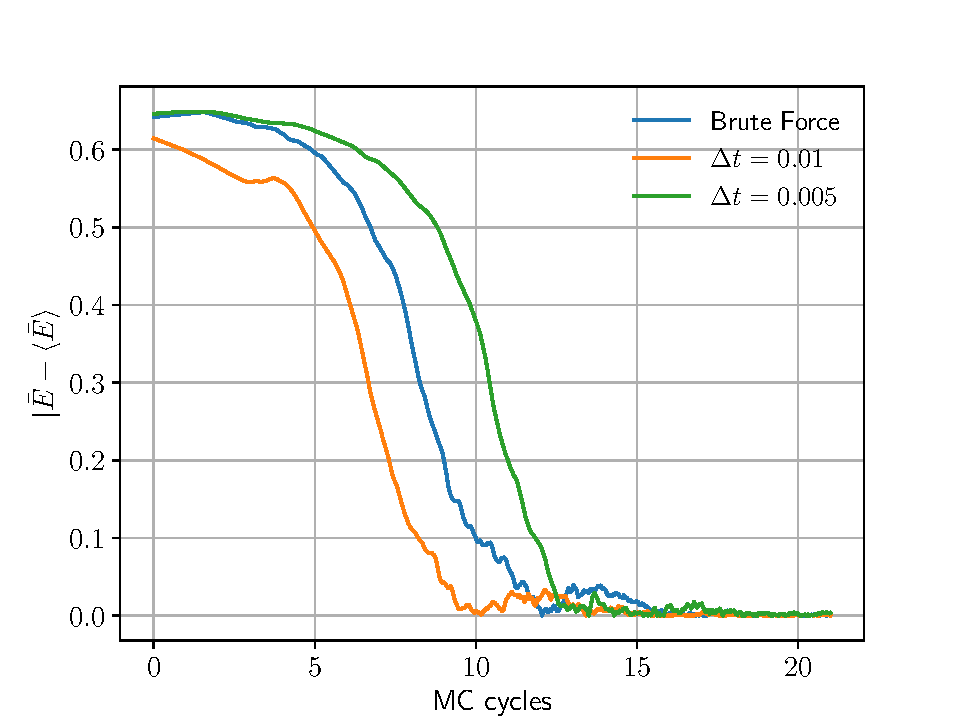
\includegraphics[scale=0.6]{../Results/convergence_dt.pdf} 
        \caption{Non-interacting. Average energy deviation from mean over $10$ runs of $N=10$, $d=3$,$\alpha=0.45$, for brute force, and importance sampling method with $\Delta t=0.01$ and  $\Delta t=0.005$, over as a function of Monte Carlo cycles}
        \label{fig:compare_BF_IS}   
\end{figure}  

Figure \ref{fig:compare_BF_IS} shows a comparison of the average energy deviation as a function of Monte Carlo cycles for both brute force and importance sampling. The figure indicates that importance sampling using $\Delta t=0.01$ reaches a stable value of $\bar E$ after fewer cycles than the brute force method. However, $\Delta t =0.005$ requires still more cycles than brute force force method. This suggests that importance sampling with the suitable value of $\Delta t$ may be used to decrease the number of cycles before starting to sample the local energy. On the other hand, unsuitable values of $\Delta t$ may lead to worse performance in terms of required equilibrium cycles, compared to the brute force approach.  Table \ref{table:BF_IS} shows the corresponding values for the estimation error, acceptance rate and time. Both the brute force method and the importance sampling method at $\Delta t=0.1$ show $\hat \sigma$ of order $10^{-3}$, while the $\Delta t=0.005$ has an order of magnitude larger average $\hat \sigma$ value. In this last case this is likely due to the trend described earlier about lower values of $\Delta t$. Comparing $\Delta t=0.1$ and the brute force method, the brute force method comes out on top, owing to the fact that the algorithm is faster. However, this does not imply that the brute force method is to be preferred over importance sampling in general, both because $\Delta t=0.1$ might not be the best suited value for the tested configuration and because similar tests for more complex systems are also needed, as well as other values of $\alpha$.



\begin{table}[h!]
\begin{center}
\begin{tabular}{lllll}
\hline
Method									    & $\bar E $ & $\hat \sigma$		   & $\bar A$ & $\bar t$ [ms]  \\
\hline
Brute force 								& $15.1$  		&$5.49 \times 10^{-3}$ &  $0.737$ & $7633$\\
Importance sampling ($\Delta t=0.1$)		& $15.1$ 		&$4.08 \times 10^{-3}$ &  $0.8987$ & $9503$\\
Importance sampling ($\Delta t=0.005$)		& $15.1$ 		&$1.64 \times 10^{-2}$ &  $0.999$ & $9599$\\
\hline
\end{tabular}
\end{center}
\caption{Non-interacting. Comparison of brute force and importance sampling averaged over $10$ runs of $N=10$, $d=3$, $\alpha=0.45$, at $21^3$  cycles with a $0.3$ equilibrium fraction. }
\label{table:BF_IS}
\end{table}


On the basis of the observations and discussions above, I am is unable to make any exact conclusions on the consequences of the choice of $\Delta t$, other than that the number of particles, $N$, and the value of $\alpha$, appear to effect the dependence of $\hat \sigma$ on $\Delta t$. Further more, the value of $\Delta t$ appears to effect the correlation time of the samples, to the extent where $\sigma$ as a quality measurement may be misleading. The value of $\bar E$ as well as $\hat \sigma$ must be evaluated when determining if one has used the correct $\Delta t$, and simulations requiring high precision should include some variations on $\Delta t$. When compared to the brute force method, importance sampling appears to equilibrate after fewer MC cycles than what than the brute force method, but only if $\Delta t$ is at a suitable value, which comes at the cost of increased CPU time.

\subsection{Interacting Bose gas in elliptical trap}
Having established a working implementation for multiple particles in three dimensions both using the Importance Sampling and Brute Force methods, I now move on to results from the interacting Bose gas implementation. Including particle interaction in the simulations will necessarily mean that $\alpha=0.5$ no longer produces the lowest energy for all particle systems. As such, I have chosen to closer examine the effects of using Gradient Descent (GD) to approximate $\alpha$ (initial testing of the implementation of the GD method is shown to be performing as expected in figure \ref{fig:GD} in appendix 1). After the discussion on GD, I move on to comparing interacting and non-interacting systems for various numbers of particles, before presenting a visualization of the of wave-function in terms of one-body densities. All the presented results below are produced using Importance Sampling, and the number of dimensions, $d$, is set to $3$. Unless stated otherwise, $\lambda=\sqrt{8}$. 

\begin{figure}[!h]
        \centering 
         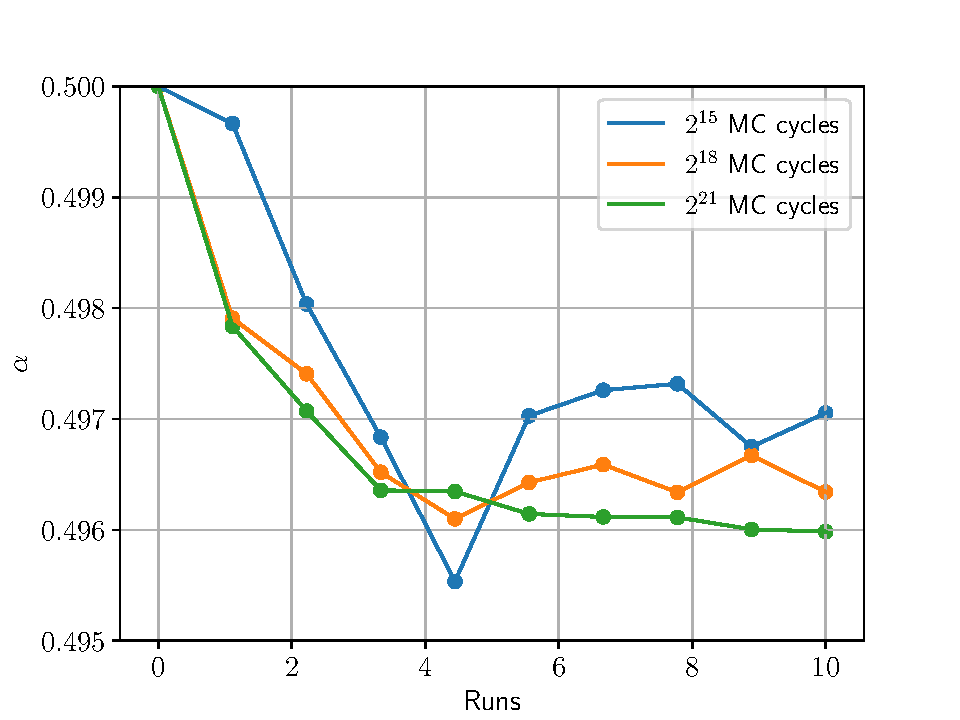
\includegraphics[scale=0.6]{../Results/Data_analysis/GD_interacting.pdf} 
        \caption{Interacting. Gradient Descent with adaptive learning rate $\eta_{k+1}= 0.9\eta_{k} $, on $\alpha$ for $N=10$ using $\Delta t=0.01$ for various numbers of MC cycles (with a $0.3$ equilibration factor).}
        \label{fig:GD_interacting}   
\end{figure}  

Figure \ref{fig:GD_interacting} shows the iterative evolution of $\alpha$ when using gradient descent for different numbers of MC cycles. It is clear from the graph that the $2^{21}$ cycles case has less variance in the produced values of $\alpha$ than the two other values, and that $2^{15}$ has the highest variance in $\alpha$ values. This may indicate that higher numbers of MC cycles give more accurate $\alpha$-gradients, as one should expect. In order to further test this, the by-eye mean of $\alpha$ for $2^{21}$ cycles and $2^{15}$ and $2^{18}$ cycles, $\alpha=0.496$ and $\alpha=0.4965$ respectively, were used in $10$ runs with $2^{21}$ cycles (table \ref{table:alpha_compare}). The table shows that $\hat \sigma$ for $\alpha=0.4960$ is of order $10^{-5}$ 
smaller than for $\alpha=0.4965$, simultaneously $\bar E$ is smaller in the $\alpha=0.4965$ case, by a magnitude of $10^{-3}$. This inconsistency is likely caused by having used too few experiments, that the parameter values are too similar to produce easily interpreted results, and/or that the accuracy limit of the current implementation is reached before discrepancies of order $10^{-4}$ in $\alpha$ becomes evident. 


\begin{table}[h!]
\begin{center}
\begin{tabular}{lllll}
\hline
$\alpha$					& $\bar E $     & $\hat \sigma$		    \\
\hline
$0.4960$			& $24.3993$ 		&$9.99 \times 10^{-4}$ \\
$0.4965$			& $24.3986$ 		&$8.69 \times 10^{-4}$ \\
\hline
\end{tabular}
\end{center}
\caption{Interacting. Comparison between $\alpha$ values based on figure \ref{fig:GD_interacting}, of averages over $10$ runs, using $2^{21}$ MC cycles and $\Delta t=0.1$.}
\label{table:alpha_compare}
\end{table}


\begin{table}[h!]
\begin{center}
\begin{tabular}{l|l|l|l|l|l|l|l|l} \hline
\multirow{2}{*}{\begin{tabular}{c} $N$ \end{tabular}} & \multicolumn{4}{c|}{Interacting} & \multicolumn{4}{c}{Non-interacting}\\ \cline{2-9}
	    			& $\bar E$ 		&$\bar E/N$	& $\hat \sigma$ 		&time[$s$]& $\bar E$  			& $\bar E/N$	& $\hat \sigma$ 		&time[$s$]\\ \hline 
$10(\alpha=0.496)$  & $24.399$		&$2.440$	& $2.87	\times 10^{-3}$	& $4 $		& $24.349$		  		& $2.435$		& $9.01 \times 10^{-3}$ 	&$1$\\
$50(\alpha=0.457)$  & $127.267$		&$2.545$	& $4.05 \times 10^{-2}$ & $50 $		& $123.312$				& $2.466$ 		&$7.18 \times 10^{-2}$  	&$4$\\
$100(\alpha=0.494)$ & $266.150$		&$2.662$	& $1.33 \times 10^{-1}$ & $190 $		& $244.630$				& $2.446$ 		&$1.6 \times 10^{-1}$   &$9$\\ \hline
\end{tabular}
\end{center}
\caption{Comparison between interacting and non-interacting systems using $\alpha$ from GD and $\beta=\gamma=2.82843$. The values are averages over $10$ runs, using $2^{18}$ MC cycles and $\Delta t=0.01$.}
\label{table:interacting_noninteracting}
\end{table}

Table \ref{table:interacting_noninteracting} shows the estimated energy $\bar{E}$, estimated energy per particle $\bar E /N$, error estimate using blocking, $\hat \sigma$, and CPU time in seconds for different numbers of particles, with and without particle interaction, using elliptical harmonic oscillator potential, $\beta=\gamma=2.82843$. Firstly, it is clear that the ground energy of the elliptical trap is substantially higher than for the spherical trap, which is to be expected when for example looking at the Hamiltonian of the scaled system \eqref{eq:scaled_H}. Secondly, as $N$ increases, the table shows that the error estimate increases from $\hat \sigma \sim 10^{-3}$ ($N=50$) to $\sim 10^{-2}$ ($N=50$) and $\sim 10^{-1}$ ($N=100$) both with and without the Jastrow factor. However, this does not dilute the validity of the following observations on $\bar E/N$ as $\hat \sigma$ scales to $N$ at a slower rate. Comparing the different values of $N$ in the non-interacting case, it is clear that the $\bar E/N\approx 2.45\approx$ constant due to the system being a superposition of the single-particle systems of each particle. When also encompassing particle interaction however, $\bar E/N$ increases as the number of interactions on each particle is strengthened, from $\bar E/N\approx2.55$ in the case of $N=50$ to $\bar E/N\approx2.66$ for $N=100$. As such, it is evident that the inclusion of the Jastrow factor is increasingly important for higher values of $N$. Even though the error estimate increases drastically from $\hat \sigma \sim 10^3$ ($N=10$)  to $\sim 10^2$ ($N=50$) and $\sim 10^{-1}$ ($N=100$), this has only minor impact on $\bar E/N$, as $\bar E$ also increases .
  

In the interacting case, the CPU time per run increases by a factor $\sim 50$ from $N=10$ to $N=100$, while in the non-interacting case, the time increase is $\sim 10$ for the same increase in particles. As the inclusion of the Jastrow factor becomes increasingly important for higher numbers of particles, this also means that optimization is especially important when simulating higher numbers of particles. The error estimates increase with $N$, both due to increased truncation as well as a decreased number of average MC cycle per particle. Although the error estimates are of the same magnitude in both the interacting and non-interacting case, the interacting system yields in general a higher error on the estimated ground energy, possibly due to more truncation following the increased complexity of the local energy expression. As such, achieving results with a specific desired accuracy will most likely require increasing the number of Monte Carlo cycles as $N$ is increased.

The $\alpha$-values used in producing table \ref{table:interacting_noninteracting} were obtained by Gradient Descent over $10$ runs prior to the runs used in making the table. As the $\alpha$ gradient from each of these preliminary parameter runs is based on one run, the $\hat \sigma$ value in each such run directly reflects upon the variance in GD over time, meaning that $N$ large will results in less accurate estimates on $\alpha$, which again means a larger $\hat \sigma$ when calculating $\bar E$. In other words, as $N$ increases, it becomes increasingly difficult to make a decent estimation of $\alpha$, leading to increased error. This can possibly remedied to some extent by using a high number of cycles in each run when using GD. However, as $N$ and $\alpha$ both affect which value of $\Delta$ should be used in the Metropolis algorithm, this becomes a challenge indeed. Because there are many parameters involved in the VMC engine, and because, as has been shown above, several of them interact with regards to the error estimate, these types of simulations are well suited for machine learning methods. 

\begin{figure}[!h]
        \centering 
         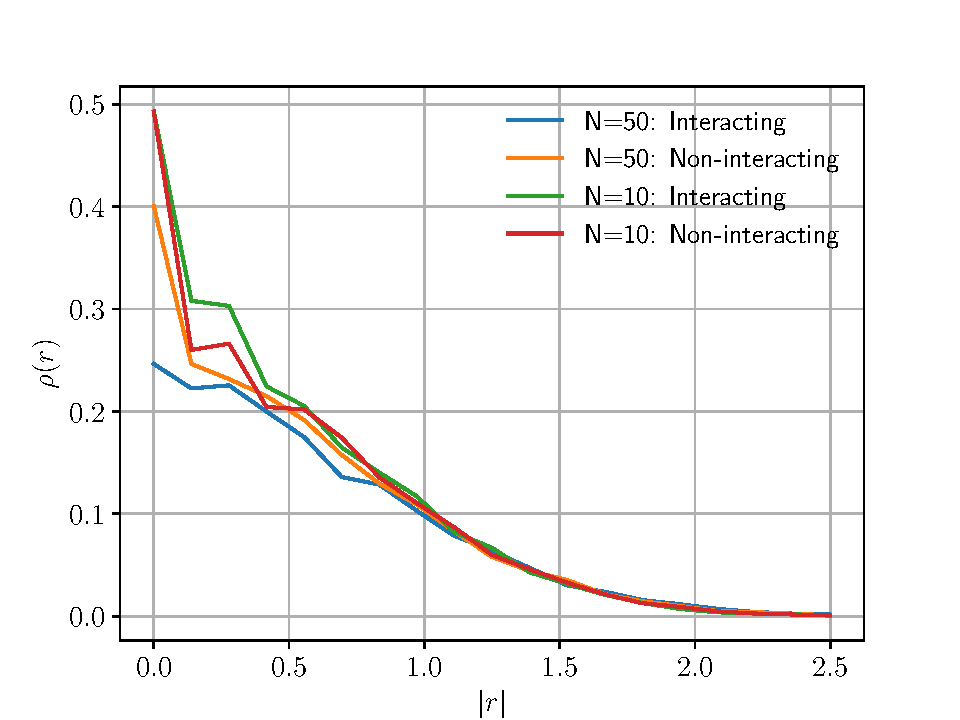
\includegraphics[scale=0.6]{../Results/Densitites/densitites_plot.pdf} 
        \caption{Bose gas in spherical trap, $\lambda=1$; One-Body density, $\rho(r)$ for $N=10$ and $N=50$, both interacting and non-interacting. The data is averaged from $7500$ particles total for each plot using importance sampling ($\Delta t=0.1$) after $2^{15}$ runs.}
        \label{fig:densities}   
\end{figure}  

Figure \ref{fig:densities} shows the one-body densities \cite{Hogberget}, which serves as a visualization of wave-functions, for $N=10$ and $N=50$, with and without the Jastrow factor/particle interaction. The figure indicates that the $N=10$ systems and the non-interacting $N=50$ case have somewhat higher one-body densities in the region $r=[0,1.0]$ than in the $N=50$ interacting case. In the case of the $N=50$ interacting system, the lower one-body density in the this region is most likely due to the combination of a relative high number of particles and the inclusion of the repulsive potential. After all, as the particles are in a three dimensional room, the available volume in $r=[0,1.0]$ for example is significantly less that than in region $r=[1.0,2.0]$. In the $N=10$, $a>0$ case, there are likely too few particles for the repulsive potential to make a significant change on the distribution of particles. Because $\rho(r)=H(r)/r^2$, differences in particle numbers for larger values of $r$ will be less visible than difference for smaller values of $r$ - which explains why the one-body density of the $N=50$ interacting case is not visibly higher for $r>1.0$, as the lower density in the $r<1.0$ region most definitely implies. 

\section{Conclusions} \label{conclusions}
Based on the results and discussion above, it is clear that the error estimate, $\sigma$, on correlated data without methods such as "blocking" is large deceptive. In most cases, the error estimate using "blocking", $\hat \sigma$, was entirely necessary, such as when studying the effect of $\Delta t$ used in the Importance Sampling method on estimation quality of $\bar E$. In this project, I used "blocking" post-simulation in a separate Python implementation, which encumbered the analysis of the results severely. Similar research in the future will in my opinion benefit from implementing the required error analysis in such a way that it may be be executed effectively in sequence with generating the data samples.  

The presented results indicated that Importance Sampling may accelerate the equilbration of the system due to a higher acceptance rate $A$, enabling simulations with fewer Monte Carlo cycles than when using the Brute Force Monte Carlo integration. This requires finding a suitable $\Delta t$ value, as some of the tested values were shown to equilibrate the local energy $E_L$ slower than the Brute Force method, and accepting nearly all proposed particle configurations, leading to a larger error estimate $\hat \sigma$.  Without the Jastrow factor, for $N=10$ $\alpha=0.45$ after $2^{21}$ MC cycles, $\Delta t=0.1$ produced an average $\hat \sigma \sim 10^{-3}$ ($A=0.9$), which was the same order of magnitude as the Brute Force method, which had $A=0.74$. Simultaneously, $\Delta t=0.005$ resulted in $\hat \sigma \sim 10^{-2}$ with $A \approx 1$. 

Increases in particle number $N$ was generally observed to increase $\hat \sigma$. After $2^{18}$ cycles $\hat \sigma \sim 10^3$ ($N=10$) increased to $\sim 10^2$ ($N=50$) and $\sim 10^{-1}$ ($N=100$), both with and without the Jastrow factor. This did not however impact on the validity of the results on average estimated energy per particle, $\bar E/N$ as $\hat \sigma$ scaled to $N$ at a slower rate than $\bar E$. When including the Jastrow factor however, $\bar E/N$ increased from $\bar E/N\approx2.45\approx$ constant for all values of $N$, to $4.55$ ($N=50$) and $2.66$($N=100$). Based on this, I concluded that the Jastrow factor is increasingly important for higher values of $N$, which was further underlined by studying the one-body density of systems of $N=50$ and $N=100$ particles.

The simulations performed in this project have to some extent yielded results that were difficult if not impossible to draw any definite conclusions from. This has largely been due to the stochasticity introduced through the Monte Carlo algorithms, which for some purposes require averaging a high number of simulations in order to study the finer nuances. The large number of parameters involved ($N$, $\Delta t$, $\alpha$, $\eta$, etc.) have further complicated interpreting the results. Due to this, further study focusing on certain aspects such as; the effect of the approximation of $\alpha$ on the optimal $\Delta t$, one-body densities in the $r\rightarrow 0$ limit, or the impact of $N$ on the best suited $\Delta t$ have been only been studied cursory. More elaborate and focused research than what is encompassed by the scope of this project is therefore required in order to make any conclusions on those subjects. Furthermore, the time required to run each simulation went from $\sim 10^0$ ($N=10$) seconds to $10^2$ ($N=100$). As such, I find that VMC is well suited for application of Machine Learning methods, especially in tandem with well optimized and parallelized code. 

\bibliography{ref} \label{refer}
\bibliographystyle{plain}


\begin{appendices}
\section{Appendix 1.} \label{APP_1}
\begin{table}[h!]
\begin{center}
\begin{tabular}{llll}
\hline
 $\alpha$ & $\bar{E} $ & $\hat \sigma$ & $t (ms)$ \\
\hline
$0.30$ 	  & $5.69$ & $1.94 \times 10^{-2}$ &  - \\  
$0.35$ 	  & $5.34$ & $1.19 \times 10^{-2}$ & -  \\  
$0.40$ 	  & $5.14$ & $6.94 \times 10^{-3}$ & -  \\  
$0.45$ 	  & $5.03$ & $3.12 \times 10^{-3}$ & -  \\  
$0.50$ 	  & $5.00$ & $0.00$ & -  \\  
$0.55$ 	  & $5.02$ & $2.65 \times 10^{-3}$ & -  \\  
$0.60$ 	  & $5.08$ & $4.88 \times 10^{-3}$ & -  \\  
$0.65$ 	  & $5.17$ & $6.19 \times 10^{-3}$ & -  \\  
$0.70$ 	  & $5.27$ & $8.16 \times 10^{-3}$ & -  \\  
Average   &    -	& $7.15 \times 10^{-3}$ & $2661$\\
\hline
\end{tabular}
\end{center}
\caption{$N=10$, $D=1$ after $2^{21}$ cycles, with a $0.3$ equilibrium fraction, for various values of $\alpha$.}
\label{table:N10D1}
\end{table}

\begin{figure}[!h]
        \centering 
         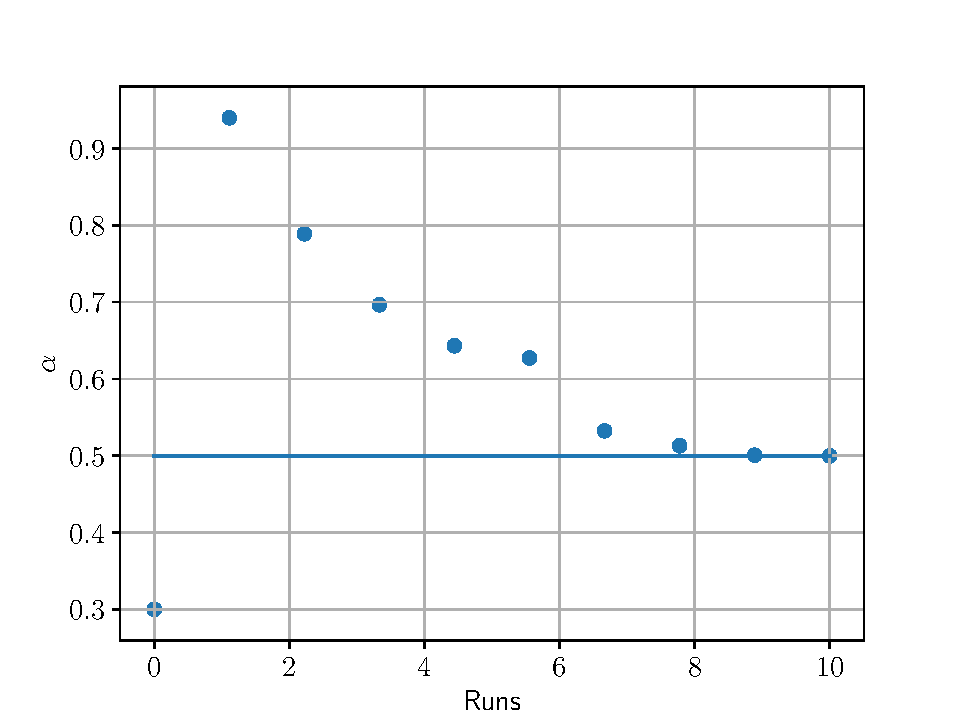
\includegraphics[scale=0.6]{../Results/Data_analysis/GD.pdf} 
        \caption{Non-interacting case. Gradient Descent on $\alpha$ for $N=100$, $d=3$, using importance sampling ($\Delta t=0.1$)}
        \label{fig:GD}   
\end{figure}  


\section*{Appendix 2.} \label{APP_2}
\subsection*{Analytic local energy, non-interacting spherical} \label{APP_2:le_1}
Gradient of $g$:
\begin{equation*}
{\nabla }_{i} g(\alpha,\beta,\mathbf{r}_i)=-2\alpha(\bm x + \bm y+ \beta \bm z) g(\alpha,\beta,\mathbf{r}_i)
\end{equation*}
Laplacian of $g$:
From the product rule, derivation of $ \mathbf{r}_i$, gives a coefficient $d$ representing the dimensionality of $r$. 
\begin{equation*}
{\nabla }_{i}^2  g(\alpha,\beta,\mathbf{r}_i)=  (-2(d-1+\beta) \alpha  + 4 \alpha^2  (x^2 + y^2 + \beta^2 z^2)) g(\alpha,\beta,\mathbf{r}_i)
\end{equation*}
Meaning that in the $\beta=1$ case,
\begin{equation*}
        E_L(\mathbf{r}) =  \sum_i^N \left(\frac{-\hbar^2}{2m}(-2 d \alpha + 4 \alpha^2  \mathbf{r}_i^2) + \frac{1}{2}m\omega_{ho}^2r_i^2 )\right)  
 \end{equation*}
Using natural units, $\hbar=c=1$, and unity mass $m=1$, the equation becomes;

\begin{equation*}
        E_L(\mathbf{r}) =  \alpha d N + \left( - 2 \alpha^2    + \frac{1}{2} \omega_{ho}^2\right)  \sum_i^N r_i^2 
\end{equation*}

And using the gradient of $g$, the drift force is
\begin{equation*}
F_i = \frac{2\nabla \Psi_T}{\Psi_T}= -4\alpha \mathbf{r}_i 
\end{equation*}

\subsection*{Analytic local energy, interacting eliptical} \label{APP_2:le_2}
Starting with
\begin{equation*}
    E_L(\mathbf{r}) =\frac{1}{ 
    \left[
    \prod_i \phi_i
\right]
\exp{\left(\sum_{j<k}u_{jk}\right)}
}  \sum_i^N \left(\frac{-\hbar^2}{2m}{\nabla }_{i}^2 +\frac{1}{2}m\omega_{ho}^2r^2 \right)  \left[
    \prod_i \phi_i
\right]
\exp{\left(\sum_{j<k}u_{jk}\right)}
 \end{equation*}
With the first goal being to calculate the term
\begin{equation*}
   \frac{1}{\Psi_T(\mathbf{r})}\sum_i^{N}\nabla_i^2\Psi_T(\mathbf{r}),
\end{equation*}
starting by taking the gradient with respect to the k'th particle;
\begin{align*}
  \nabla_k\Psi_T(\mathbf{r}) &= \nabla_k \left(\left[
    \prod_i \phi_i
\right]
\exp{\left(\sum_{j<m}u_{jm}\right)}\right) \\
 &= \left( \nabla_k \left[
    \prod_i \phi_i
\right] \right)
\exp{\left(\sum_{j<m} u_{jm}\right)} +
\left[
    \prod_i \phi_i
\right]
\left( \nabla_k \exp{\left(\sum_{j<m} u_{jm} \right)}\right) \label{AA_gradfullTW}
\end{align*}
The gradient of the non-interacting part of the TW:
\begin{align}
\begin{split}
& \nabla_k \left[
    \prod_i \phi_i
\right] =  \nabla_k \phi_k \left[
    \prod_{i\neq k} \phi_i
\right]= \nabla_k \phi_k \frac{\prod_i g(\alpha,\beta,\mathbf{r}_i)}{\phi_k} \\
\end{split}
\end{align}
And the gradient of the interacting part, remembering that $r_{kl}=r_{lk}$;
\begin{align}
\nabla_k \exp{\left(\sum_{j<m} u_{jm} \right)}
= \exp{\left(\sum_{j<m} u_{jm} \right)} \sum_{j\neq k} \nabla_k u_{kj}
=  \prod_{j<m} f(r_{jm}) \sum_{l\neq k} \nabla_k u_{kl}
\end{align}

Thus \eqref{AA_gradfullTW} is
\begin{align}
\begin{split}
  \nabla_k\Psi_T(\mathbf{r}) &= \nabla_k\phi_k\left[\prod_{i\ne k}\phi_i\right]\exp{\left(\sum_{j<m}u_{jm}\right)}
  \\
  &\qquad
  +  \left[\prod_i\phi_i\right]
  \exp{\left(\sum_{j<m}u_{jm}\right)}\sum_{l\ne k}\nabla_k u_{kl}
\end{split}
\end{align}
or

\begin{align}
\begin{split}
  \nabla_k\Psi_T(\mathbf{r}) &=\nabla_k \phi_k \frac{\prod_i g(\alpha,\beta,\mathbf{r}_i)}{\phi_k}\prod_{j<m} f(r_{jm})
  \\
  &\qquad
  +  \prod_i  g(\alpha,\beta,\mathbf{r}_i)
 \prod_{j<m} f(r_{jm})\sum_{l\ne k}\nabla_k u_{kl} \\
&= \left(\ \frac{\nabla_k \phi_k}{\phi_k} + \sum_{l\ne k}\nabla_k u_{kl} \right) \Psi_T(\mathbf{r})  
\end{split}
\label{eq:A1_gradpsi}
\end{align}
Next, the above expressions are used to find the second derivative;

\begin{align}  
\begin{split}
\frac{1}{\Psi_T(\mathbf{r})} \nabla_k^2\Psi_T(\mathbf{r}) 
&=
\frac{1}{\Psi_T(\mathbf{r})} \nabla_k\left( \left(\frac{\nabla_k \phi_k}{\phi_k} + \sum_{l\ne k}\nabla_k u_{kl} \right) \Psi_T(\mathbf{r}) \right)\\
&=
\frac{1}{\Psi_T(\mathbf{r})} \left(\left(\phi_k \nabla_k\frac{1}{\phi_k} +\frac{\nabla_k^2 \phi_k}{\phi_k} + \sum_{l\ne k}\nabla_k^2 u_{kl} \right)\Psi_T(\mathbf{r}) + 
\left(\ \frac{\nabla_k \phi_k}{\phi_k} + \sum_{l\ne k}\nabla_k u_{kl} \right)^2 \Psi_T(\mathbf{r})   \right) \\
&=
 \left(\ \frac{\nabla_k \phi_k}{\phi_k} \right)^2 + \frac{\nabla_k^2 \phi_k}{\phi_k} + \sum_{l\ne k}\nabla_k^2 u_{kl}  + 
\left(\ \frac{\nabla_k \phi_k}{\phi_k} + \sum_{l\ne k}\nabla_k u_{kl} \right)^2 \\
&=
 -\left(\frac{\nabla_k \phi_k}{\phi_k}\right)^2 + \frac{\nabla_k^2 \phi_k}{\phi_k} + \sum_{l\ne k}\nabla_k^2 u_{kl}  + 
\left(\ \frac{\nabla_k \phi_k}{\phi_k} \right)^2 + 2\left(\ \frac{\nabla_k \phi_k}{\phi_k} \sum_{l\ne k}\nabla_k u_{kl} \right)+ \left(\ \sum_{l\ne k}\nabla_k u_{kl} \right)^2 \\
&= 
\frac{\nabla_k^2 \phi_k}{\phi_k} + 2  \frac{\nabla_k \phi_k}{\phi_k} \sum_{l\ne k}\nabla_k u_{kl} + \sum_{l\ne k}\nabla_k^2 u_{kl}   + \left(\ \sum_{l\ne k}\nabla_k u_{kl} \right)^2
\end{split}      
\end{align}
In order to simplify applying the $\nabla_k$-operator to $u_{kl}$, the operator is re-written:
\begin{align*}
\nabla_k = \nabla_k \frac{\partial r_{kl}}{\partial r_{kl}} = \nabla_k \sqrt{\left(\bm r_k - \bm r_l \right)^2} \frac{\partial}{\partial r_{kl}} = \frac{\bm r_k - \bm r_l}{r_{kl}} \frac{\partial}{\partial r_{kl}}
\end{align*}
This re-written operator is then applied to the $\nabla_k u_{kl}$ terms, such that
\begin{align*}
\nabla_k u_{kl} = \frac{\bm r_k - \bm r_l}{r_{kl}} \frac{\partial u_{kl}}{\partial r_{kl}} = \frac{\bm r_k - \bm r_l}{r_{kl}}  u'_{kl}
\end{align*}
And
\begin{align*}
\nabla_k^2 u_{kl} 
&= \left( \nabla_k  \frac{\bm r_k - \bm r_l}{r_{kl}} \right) \partial u'_{kl}  +  \frac{\bm r_k - \bm r_l}{r_{kl}} \left( \nabla_k   u'_{kl}  \right) \\
&=  \left( \frac{ \nabla_k (\bm r_k - \bm r_l)}{r_{kl}} \right)  u'_{kl}  +   (\bm r_k - \bm r_l) \left( \nabla_k \frac{1 }{r_{kl}} \right)  u'_{kl}  +  \frac{\bm r_k - \bm r_l}{r_{kl}} \left( \nabla_k   u'_{kl}  \right) \\
&= 
\frac{d}{r_{kl}}   u'_{kl}  -  (\bm r_k - \bm r_l) \frac{(\bm r_k - \bm r_l)}{r_{kl}^3}   u'_{kl} 
+  \left( \frac{\bm r_k - \bm r_l}{r_{kl}} \right)^2   u{''}_{kl} \\
&= 
\left( \frac{d}{r_{kl}}   -   \frac{(\bm r_k - \bm r_l)^2}{r_{kl}^3} \right)  u'_{kl} 
+  \left( \frac{\bm r_k - \bm r_l}{r_{kl}} \right)^2   u{''}_{kl}
\end{align*}
Where $(\bm r_k - \bm r_l)^2={r_{kl}}^2$, thus
\begin{align*}
\nabla_k^2 u_{kl} 
&=
\left( \frac{d}{r_{kl}}   -   \frac{1}{r_{kl}} \right)  u'_{kl} 
+    u{''}_{kl} =   \frac{d-1}{r_{kl}}   u'_{kl} 
+    u{''}_{kl}
\end{align*}
Applied to the Laplacian;
\begin{align}
\begin{split}
\frac{1}{\Psi_T(\mathbf{r})} \nabla_k^2\Psi_T(\mathbf{r}) 
&=
\frac{\nabla_k^2 \phi_k}{\phi_k} + 2  \frac{\nabla_k \phi_k}{\phi_k} \sum_{l\ne k}\frac{\bm r_k - \bm r_l}{r_{kl}}  u'_{kl}  \\
&+  \left(\ \sum_{l\ne k} \frac{\bm r_k - \bm r_l}{r_{kl}} \partial u'_{kl} \right)^2 \\
&+ \sum_{l\ne k} \left( \frac{d-1}{r_{kl}}   u'_{kl} +   u{''}_{kl} \right)
\end{split}
\end{align}
Expanding the third term, re-arranging, and inserting $d=3$;
\begin{align}
\begin{split}
\frac{1}{\Psi_T(\mathbf{r})} \nabla_k^2\Psi_T(\mathbf{r}) 
&=
\frac{\nabla_k^2 \phi_k}{\phi_k} + 2  \frac{\nabla_k \phi_k}{\phi_k} \sum_{l\ne k}\frac{\bm r_k - \bm r_l}{r_{kl}}  u'_{kl}  \\
&+  \sum_{j\ne k} \sum_{l\ne k} \frac{(\bm r_k - \bm r_l)(\bm r_k - \bm r_j)}{r_{kj} r_{kl} }  u'_{kj}  u'_{kl} \\
&+ \sum_{l\ne k} \left(   u{''}_{kl} + \frac{2}{r_{kl}}   u'_{kl} \right)
\end{split}
\end{align}

For the drift Force;
Using \eqref{eq:A1_gradpsi}, the drift force of for particle $k$ in the interacting system
\begin{equation*}
F_k = \frac{2\nabla \Psi_T}{\Psi_T}= 2 \left(\ \frac{\nabla_k \phi_k}{\phi_k} + \sum_{l\ne k}\nabla_k u_{kl} \right) 
\end{equation*}




\end{appendices}



\end{document}